
%
% state - mapping stack
%

\section{A Modern Web Mapping Stack}
\label{chapter:web-mapping-stack}

The primary purpose of web mapping applications is to deliver spatial data in the form of a map to the user. Modern, interactive web mapping applications are based on a concept named \textit{slippy maps}. These maps are brought to the user by a combination of client- and server-side technologies. Figure \ref{fig:web-mapping-stack} illustrates the prototype of such a modern web mapping application. Similar mapping stacks are documented in 
\cite{Schuetze07smart, mitchell2008web, Miler10webis, McArdle10arch}. Its components will be discussed in the following section.


\begin{figure}[h]
  \begin{center}
    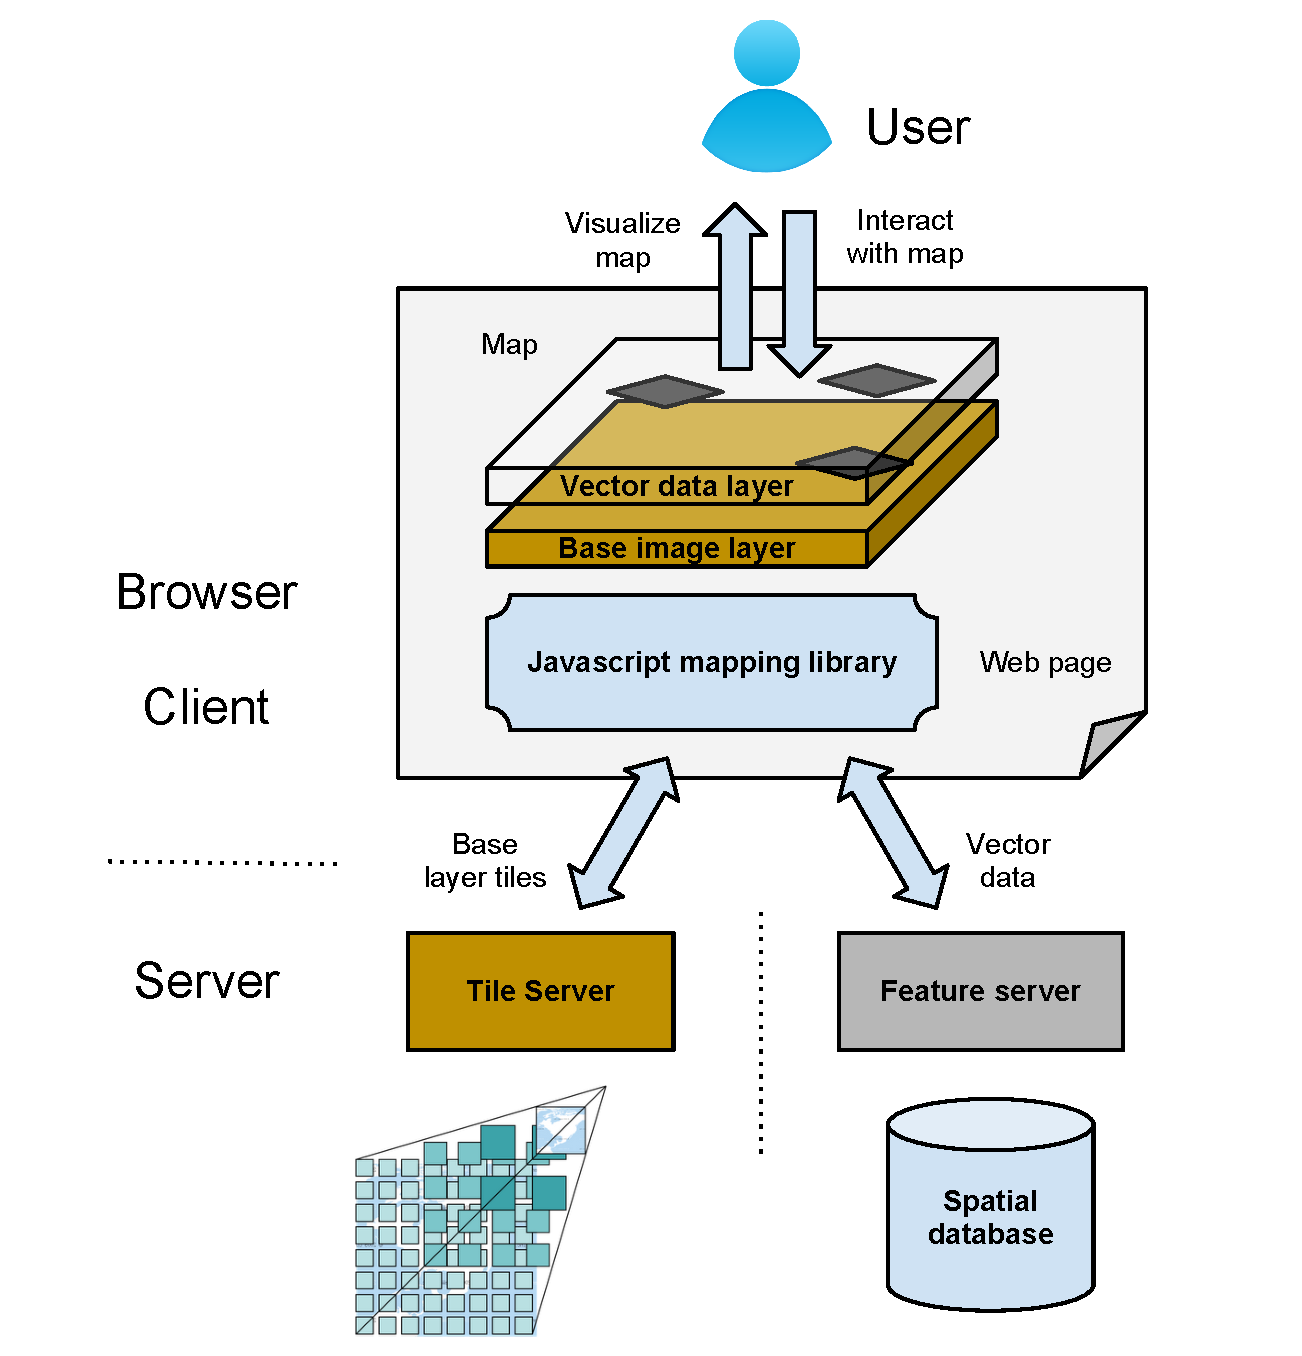
\includegraphics[width=1\textwidth]{figures/web_mapping_stack.pdf}
    \caption{Illustration of a modern web mapping application. Includes a tile graphic from~\cite{web:cubeservtiles}.}
    \label{fig:web-mapping-stack}
  \end{center}
\end{figure}


\begin{itemize}

\item A \textbf{slippy map} is displayed to the user in a rectangular viewport within the browser and handled by a JavaScript mapping library. The map is visualized dynamically by rendering layers of raster and vector data on top of each other. In addition, the slippy map provides means of interaction to the user such as panning and zooming to update and explore the map. 

\item A \textbf{JavaScript mapping library} is in charge of rendering the slippy map by positioning one or multiple layers on top of each other. Usually, a base layer of raster data is combined with a vector data layer on top of it. Current JavaScript mapping libraries include \textit{OpenLayers}\footnote{\url{http://openlayers.org/}}, \textit{Leaflet}\footnote{\url{http://leafletjs.com/}} and \textit{Modest Maps}\footnote{\url{http://modestmaps.com/}}.

\item A \textbf{tile server} provides static, sliced-up images of the raster image data for creating base layers of the slippy map. The JavaScript mapping library requests on these tiles on demand, based on the current viewport. When the user performs actions like dragging and zooming on the map, the current viewport will get changed. The JavaScript library then requests additional data from the server, if needed and updates the map accordingly. This live-updating process is also referred to as \textit{Bounding Box Strategy} (BBOX Strategy)\footnote{\url{http://openlayers.org/dev/examples/strategy-bbox.html}}. Standards for consuming tiles include \textit{Web Map Service} (WMS)\footnote{\url{http://en.wikipedia.org/wiki/Web_Map_Service}} and \textit{Tile Map Service} (TMS)\footnote{\url{http://en.wikipedia.org/wiki/Tile_Map_Service}}.

A typical tile set represents $256 \times 256$ pixel tiles of the whole world at 18 zoom levels. The fact that this leads to billions of tiles has created its own line of businesses. Map providers like \textit{Google Maps}\footnote{\url{http://maps.google.com/}} and \textit{Stamen}\footnote{\url{http://maps.stamen.com/}} both offer default base layers and also allow users to create their own custom tile sets. \textit{TileMill}\footnote{\url{http://mapbox.com/tilemill/}} is an open source project that allows users to design their own custom maps using a design studio. The resulting maps can either be self-hosted on a server by using its complement \textit{TileStream}\footnote{\url{https://github.com/mapbox/tilestream}} or imported into \textit{MapBox Hosting}\footnote{\url{http://mapbox.com/hosting}}.  

\item A \textbf{feature server} provides vector data to the JavaScript mapping library in an analogous way as the tile server does. Note the difference: while raster data will be displayed directly as an image, the vector data gets rendered on the client-side.

To provide dynamic data, the feature server usually relies on a \textit{spatial database}. Spatial extensions exist for various databases, including \textit{PostGis}\footnote{\url{http://en.wikipedia.org/wiki/PostGIS}} and \textit{MySQL Spatial Extensions}\footnote{\url{http://dev.mysql.com/doc/refman/5.0/en/spatial-extensions.html}} and \textit{Spatialite}\footnote{\url{http://www.gaia-gis.it/gaia-sins/}}.

\end{itemize}










